\begin{titlepage}
	\begin{center}
		\vspace{1cm}

		\LARGE\chapfont{Riemann surfaces}

		\vspace{1.0cm}

		% \normalsize\rm An analytic approach to Riemann surfaces, and the
		% Riemann-Roch theorem for compact Riemann surfaces.

		\vspace{0.5cm}

		\normalsize\sc{Samuel Ireson}

		\vfill

		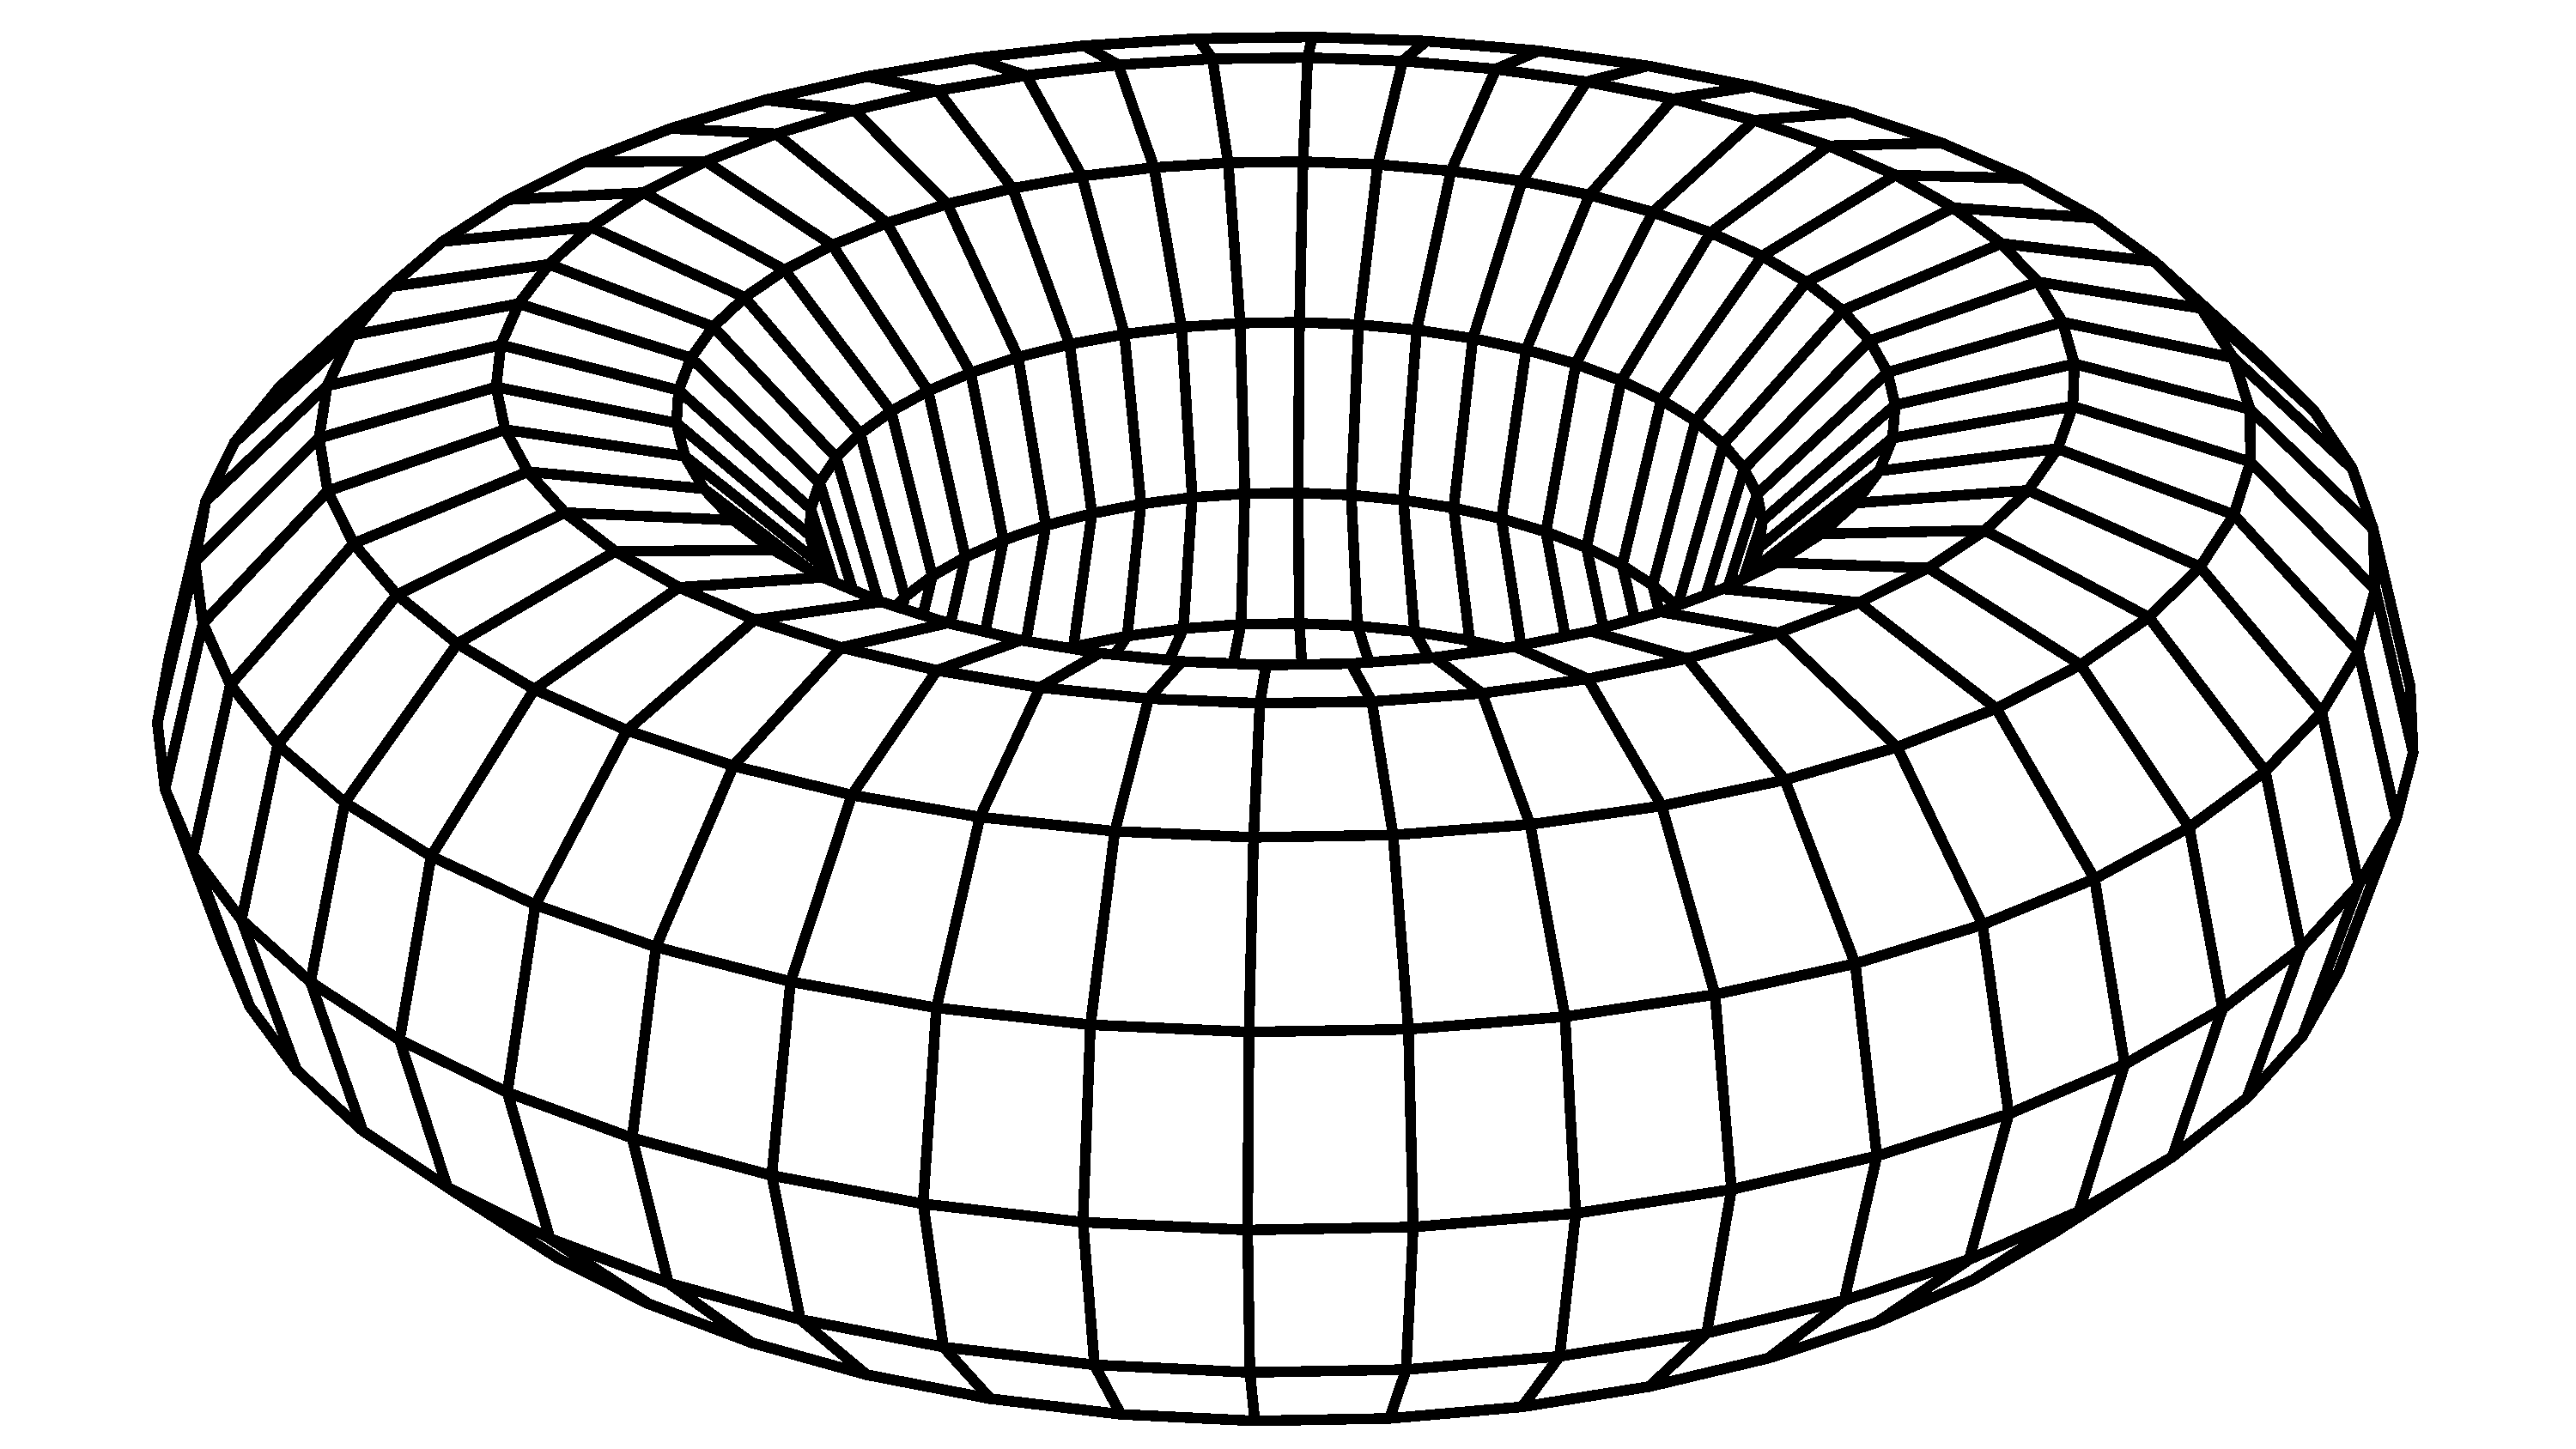
\includegraphics[width=\textwidth]{titlepage.pdf}

		\vfill

		Project III

		\vspace{0.5cm}

		Department of Mathematical Sciences

		\vspace{0.5cm}

		Durham University

	\end{center}

\end{titlepage}

\clearpage
\begin{center}
	% \thispagestyle{empty}
	\vspace*{\fill}
	For Mum,

	for Dad,

	{\accentfont за Девче}
	\vspace*{\fill}
\end{center}
\clearpage

% \thispagestyle{empty}
\vspace*{\fill}
This piece of work is a result of my own work and I have complied with the
Department's guidance on multiple submission and on the use of AI tools.
Material from the work of others not involved in the project has been
acknowledged, quotations and paraphrases suitably indicated, and all uses of AI
tools have been declared.
\vspace*{\fill}
\clearpage

